%%%%%%%%%%%%%%%%%%%%%%%%%%%%%%%%%%%%%%%%
% datoteka diploma-vzorec.tex
%
% vzorčna datoteka za pisanje diplomskega dela v formatu LaTeX
% na UL Fakulteti za računalništvo in informatiko
%
% vkup spravil Gašper Fijavž, december 2010
% 
%
%
% verzija 12. februar 2014 (besedilo teme, seznam kratic, popravki Gašper Fijavž)
% verzija 10. marec 2014 (redakcijski popravki Zoran Bosnić)
% verzija 11. marec 2014 (redakcijski popravki Gašper Fijavž)
% verzija 15. april 2014 (pdf/a 1b compliance, not really - just claiming, Damjan Cvetan, Gašper Fijavž)
% verzija 23. april 2014 (privzeto cc licenca)
% verzija 16. september 2014 (odmiki strain od roba)
% verzija 28. oktober 2014 (odstranil vpisno številko)
% verija 5. februar 2015 (Literatura v kazalu, online literatura)

\documentclass[a4paper, 12pt]{book}
\usepackage{color}
\definecolor{orange}{rgb}{1,0.6,0}
\usepackage[utf8x]{inputenc}   % omogoča uporabo slovenskih črk kodiranih v formatu UTF-8
\usepackage[slovene,english]{babel}    % naloži, med drugim, slovenske delilne vzorce
\usepackage[pdftex]{graphicx}  % omogoča vlaganje slik različnih formatov
\usepackage{fancyhdr}          % poskrbi, na primer, za glave strani
\usepackage{amssymb}           % dodatni simboli
\usepackage{amsmath}           % eqref, npr.
%\usepackage{hyperxmp}
\usepackage[pdftex, colorlinks=true,
						citecolor=black, filecolor=black, 
						linkcolor=black, urlcolor=black,
						pagebackref=false, 
						pdfproducer={LaTeX}, pdfcreator={LaTeX}, hidelinks]{hyperref}

\usepackage{listings}     

%%%%%%%%%%%%%%%%%%%%%%%%%%%%%%%%%%%%%%%%
%	DIPLOMA INFO
%%%%%%%%%%%%%%%%%%%%%%%%%%%%%%%%%%%%%%%%
\newcommand{\ttitle}{Orodje za ročno poravnavo 2D in 3D medicinskih posnetkov}
\newcommand{\ttitleEn}{A tool for manual alignment of 2D and 3D medical recordings}
\newcommand{\tsubject}{\ttitle}
\newcommand{\tsubjectEn}{\ttitleEn}
\newcommand{\tauthor}{Jure Kolenko}
\newcommand{\tkeywords}{Muh keyword1, hue}
\newcommand{\tkeywordsEn}{Muh keyword1, hue}



\usepackage{hyperref}
%%%%%%%%%%%%%%%%%%%%%%%%%%%%%%%%%%%%%%%%
%	HYPERREF SETUP
%%%%%%%%%%%%%%%%%%%%%%%%%%%%%%%%%%%%%%%%
\hypersetup{pdftitle={\ttitle}}
\hypersetup{pdfsubject=\ttitleEn}
\hypersetup{pdfauthor={\tauthor}}
\hypersetup{pdfkeywords=\tkeywordsEn}

%%%%%%%%%%%%%%%%%%%%%%%%%%%%%%%%%%%%%%%%
% postavitev strani
%%%%%%%%%%%%%%%%%%%%%%%%%%%%%%%%%%%%%%%%  

\addtolength{\marginparwidth}{-20pt} % robovi za tisk
\addtolength{\oddsidemargin}{40pt}
\addtolength{\evensidemargin}{-40pt}

\renewcommand{\baselinestretch}{1.3} % ustrezen razmik med vrsticami
\setlength{\headheight}{15pt}        % potreben prostor na vrhu
\renewcommand{\chaptermark}[1]%
{\markboth{\MakeUppercase{\thechapter.\ #1}}{}} \renewcommand{\sectionmark}[1]%
{\markright{\MakeUppercase{\thesection.\ #1}}} \renewcommand{\headrulewidth}{0.5pt} \renewcommand{\footrulewidth}{0pt}
\fancyhf{}
\fancyhead[LE,RO]{\sl \thepage} \fancyhead[LO]{\sl \rightmark} \fancyhead[RE]{\sl \leftmark}



\newcommand{\BibTeX}{{\sc Bib}\TeX}

%%%%%%%%%%%%%%%%%%%%%%%%%%%%%%%%%%%%%%%%
% naslovi
%%%%%%%%%%%%%%%%%%%%%%%%%%%%%%%%%%%%%%%%  


\newcommand{\autfont}{\Large}
\newcommand{\titfont}{\LARGE\bf}
\newcommand{\clearemptydoublepage}{\newpage{\pagestyle{empty}\cleardoublepage}}
\setcounter{tocdepth}{1}	      % globina kazala

%%%%%%%%%%%%%%%%%%%%%%%%%%%%%%%%%%%%%%%%
% konstrukti
%%%%%%%%%%%%%%%%%%%%%%%%%%%%%%%%%%%%%%%%  
\newtheorem{izrek}{Izrek}[chapter]
\newtheorem{trditev}{Trditev}[izrek]
\newenvironment{dokaz}{\emph{Dokaz.}\ }{\hspace{\fill}{$\Box$}}

%%%%%%%%%%%%%%%%%%%%%%%%%%%%%%%%%%%%%%%%%%%%%%%%%%%%%%%%%%%%%%%%%%%%%%%%%%%%%%%
%% PDF-A
%%%%%%%%%%%%%%%%%%%%%%%%%%%%%%%%%%%%%%%%%%%%%%%%%%%%%%%%%%%%%%%%%%%%%%%%%%%%%%%

%%%%%%%%%%%%%%%%%%%%%%%%%%%%%%%%%%%%%%%% 
% define medatata
%%%%%%%%%%%%%%%%%%%%%%%%%%%%%%%%%%%%%%%% 
\def\Title{\ttitle}
\def\Author{\tauthor}
\def\Subject{\ttitleEn}
\def\Keywords{\tkeywordsEn}

%%%%%%%%%%%%%%%%%%%%%%%%%%%%%%%%%%%%%%%% 
% \convertDate converts D:20080419103507+02'00' to 2008-04-19T10:35:07+02:00
%%%%%%%%%%%%%%%%%%%%%%%%%%%%%%%%%%%%%%%% 
\def\convertDate{%
    \getYear
}

{\catcode`\D=12
 \gdef\getYear D:#1#2#3#4{\edef\xYear{#1#2#3#4}\getMonth}
}
\def\getMonth#1#2{\edef\xMonth{#1#2}\getDay}
\def\getDay#1#2{\edef\xDay{#1#2}\getHour}
\def\getHour#1#2{\edef\xHour{#1#2}\getMin}
\def\getMin#1#2{\edef\xMin{#1#2}\getSec}
\def\getSec#1#2{\edef\xSec{#1#2}\getTZh}
\def\getTZh +#1#2{\edef\xTZh{#1#2}\getTZm}
\def\getTZm '#1#2'{%
    \edef\xTZm{#1#2}%
    \edef\convDate{\xYear-\xMonth-\xDay T\xHour:\xMin:\xSec+\xTZh:\xTZm}%
}

\expandafter\convertDate\pdfcreationdate 

%%%%%%%%%%%%%%%%%%%%%%%%%%%%%%%%%%%%%%%%
% get pdftex version string
%%%%%%%%%%%%%%%%%%%%%%%%%%%%%%%%%%%%%%%% 
\newcount\countA
\countA=\pdftexversion
\advance \countA by -100
\def\pdftexVersionStr{pdfTeX-1.\the\countA.\pdftexrevision}


%%%%%%%%%%%%%%%%%%%%%%%%%%%%%%%%%%%%%%%%
% XMP data
%%%%%%%%%%%%%%%%%%%%%%%%%%%%%%%%%%%%%%%%  
\usepackage{xmpincl}
\includexmp{pdfa-1b}

%%%%%%%%%%%%%%%%%%%%%%%%%%%%%%%%%%%%%%%%
% pdfInfo
%%%%%%%%%%%%%%%%%%%%%%%%%%%%%%%%%%%%%%%%  
\pdfinfo{%
    /Title    (\ttitle)
    /Author   (\tauthor)
    /Subject  (\ttitleEn)
    /Keywords (\tkeywordsEn)
    /ModDate  (\pdfcreationdate)
    /Trapped  /False
}


%%%%%%%%%%%%%%%%%%%%%%%%%%%%%%%%%%%%%%%%%%%%%%%%%%%%%%%%%%%%%%%%%%%%%%%%%%%%%%%
%%%%%%%%%%%%%%%%%%%%%%%%%%%%%%%%%%%%%%%%%%%%%%%%%%%%%%%%%%%%%%%%%%%%%%%%%%%%%%%

\begin{document}
\selectlanguage{slovene}
\frontmatter
\setcounter{page}{1} %
\renewcommand{\thepage}{}       % preprecimo težave s številkami strani v kazalu

%%%%%%%%%%%%%%%%%%%%%%%%%%%%%%%%%%%%%%%%
%naslovnica
 \thispagestyle{empty}%
   \begin{center}
    {\large\sc Univerza v Ljubljani\\%
      Fakulteta za računalništvo in informatiko}%
    \vskip 10em%
    {\autfont \tauthor\par}%
    {\titfont \ttitle \par}%
    {\vskip 2em \textsc{DIPLOMSKO DELO\\[2mm]
    UNIVERZITETNI ŠTUDIJSKI PROGRAM PRVE STOPNJE RAČUNALNIŠTVO IN INFORMATIKA}\par}%
    \vfill\null%
    {\large \textsc{Mentor}: doc.\ dr.  Matija Marolt\par}%
    {\vskip 2em \large Ljubljana 2015 \par}%
\end{center}
% prazna stran
\clearemptydoublepage

%%%%%%%%%%%%%%%%%%%%%%%%%%%%%%%%%%%%%%%%
%copyright stran
\thispagestyle{empty}
\vspace*{8cm}
Fakulteta za računalništvo in informatiko podpira javno dostopnost znanstvenih, strokovnih in razvojnih rezultatov. Zato priporoča objavo dela pod katero od licenc, ki omogočajo prosto razširjanje diplomskega dela in/ali možnost nadaljne proste uporabe dela. Ena izmed možnosti je izdaja diplomskega dela pod katero od Creative Commons licenc \href{http://creativecommons.si}{http://creativecommons.si}

Morebitno pripadajočo programsko kodo praviloma objavite pod, denimo, licenco 
\emph{GNU General Public License, različica 3}. Podrobnosti licence so dostopne na spletni strani \href{http://www.gnu.org/licenses/}{http://www.gnu.org/licenses/}.

\begin{center}
\mbox{}\vfill
\emph{Besedilo je oblikovano z urejevalnikom besedil \LaTeX.}
\end{center}
% prazna stran
\clearemptydoublepage

%%%%%%%%%%%%%%%%%%%%%%%%%%%%%%%%%%%%%%%%
% stran 3 med uvodnimi listi
\thispagestyle{empty}
\vspace*{4cm}

\noindent
Fakulteta za računalništvo in informatiko izdaja naslednjo nalogo:
\medskip
\begin{tabbing}
\hspace{32mm}\= \hspace{6cm} \= \kill




Tematika naloge:
\end{tabbing}
Fiddy diddling.
\vspace{15mm}

\vspace{2cm}

% prazna stran
\clearemptydoublepage

%%%%%%%%%%%%%%%%%%%%%%%%%%%%%%%%%%%%%%%%
% izjava o avtorstvu
\vspace*{1cm}
\begin{center}
{\Large \textbf{\sc Izjava o avtorstvu diplomskega dela}}
\end{center}

\vspace{1cm}
\noindent Spodaj podpisani Jure Kolenko sem avtor  diplomskega dela z naslovom:

\vspace{0.5cm}
\emph{Vizualizacija medicinskih podatkov}

\vspace{1.5cm}
\noindent S svojim podpisom zagotavljam, da:
\begin{itemize}
	\item sem diplomsko delo izdelal samostojno pod mentorstvom
		doc.\ dr.\ Matije Marolta,

	\item	so elektronska oblika diplomskega dela, naslov (slov., angl.), povzetek (slov., angl.) ter ključne besede (slov., angl.) identični s tiskano obliko diplomskega dela,
	\item soglašam z javno objavo elektronske oblike diplomskega dela na svetovnem spletu preko univerzitetnega spletnega arhiva.	
\end{itemize}

\vspace{1cm}
\noindent V Ljubljani, dne 24. avgusta 2015 \hfill Podpis avtorja:

% prazna stran
\clearemptydoublepage

%%%%%%%%%%%%%%%%%%%%%%%%%%%%%%%%%%%%%%%%
% zahvala
\thispagestyle{empty}\mbox{}\vfill\null\it%
Thanks Obama.
\rm\normalfont

% prazna stran
\clearemptydoublepage

%%%%%%%%%%%%%%%%%%%%%%%%%%%%%%%%%%%%%%%%
% posvetilo
\thispagestyle{empty}\mbox{}{\vskip0.20\textheight}\mbox{}\hfill\begin{minipage}{0.55\textwidth}%
\normalfont\end{minipage}
Posvetilo.
% prazna stran
\clearemptydoublepage

%%%%%%%%%%%%%%%%%%%%%%%%%%%%%%%%%%%%%%%%
% kazalo
\def\thepage{}% preprecimo tezave s stevilkami strani v kazalu
\tableofcontents{}


% prazna stran
\clearemptydoublepage

%%%%%%%%%%%%%%%%%%%%%%%%%%%%%%%%%%%%%%%%
% seznam kratic

\chapter*{Seznam uporabljenih kratic}

\begin{tabular}{l|l|l}
  %{\bf kratica} & {\bf angleško} & {\bf slovensko} \\ \hline
  % after \\: \hline or \cline{col1-col2} \cline{col3-col4} ...
  %{\bf CA} & classification accuracy & klasifikacijska točnost \\
\end{tabular}



% prazna stran
\clearemptydoublepage

%%%%%%%%%%%%%%%%%%%%%%%%%%%%%%%%%%%%%%%%
% povzetek
\addcontentsline{toc}{chapter}{Povzetek}
\chapter*{Povzetek}
V vzorcu je predstavljen postopek priprave diplomskega dela z uporabo okolja \LaTeX. Vaš povzetek mora sicer vsebovati približno 100 besed, ta tukaj je odločno prekratek.
\bigskip

\noindent\textbf{Ključne besede: } \tkeywords.
% prazna stran
\clearemptydoublepage

%%%%%%%%%%%%%%%%%%%%%%%%%%%%%%%%%%%%%%%%
% abstract
\selectlanguage{english}
\addcontentsline{toc}{chapter}{Abstract}
\chapter*{Abstract}
This sample document presents an approach to typesetting your BSc thesis using \LaTeX. A proper abstract should contain around 100 words which makes this one way too short.
\bigskip

\noindent\textbf{Keywords:} \tkeywordsEn.
\selectlanguage{slovene}
% prazna stran
\clearemptydoublepage

%%%%%%%%%%%%%%%%%%%%%%%%%%%%%%%%%%%%%%%%
\mainmatter
\setcounter{page}{1}
\pagestyle{fancy}

\chapter{Uvod}
\textcolor{red}{Računalniki so že dolgo pomembni za ljudi, v zadnjih časi pa še toliko bolj, saj so vedno zmogljivejši, močnejši in cenejši. Z razvojem računalnikov se je razvila tudi tehnologija za vizualizacijo, ki močno izboljša predstavo informacij v primerjavi z golimi številkami. }

\textcolor{red}{V medicini imamo množico slikovnih podatkov, ki pa jih te težko vizualizirati na zaslonu oziroma papirju, ker so objekti interesa 3 dimenzionalni (od tu dalje 3D), papir pa 2 dimenzionalen (od tu dalje 2D). Tu pride v poštev vizualizacija, tako da posnetke vidimo na zaslonu, tako kot dejansko izgledajo v realnosti.}

\textcolor{red}{Cilj moje diplomske naloge je bil narediti orodje za poravnavo 2D in 3D medicinskih podatkov, ki bi zdravnikom pomagal razbrati kje v prostoru se nahajajo deli 2D posnetka. Uporabnik naj bi izbral mrežni model ožilja in pripadajoč rentgenski posnetek, nato pa z rotiranjem in premikanjem modela oziroma slike poskrbel, da se ujemata. V naslednjem poglavju bom opisal orodja, ki sem jih uporabil, ter kako deluje sama projekcija 2D teksture na 3D model, nato pa bom opisal še kako sem nalogo implementiral kot samostojno aplikacijo, ter jo po tem integriral v že obstoječo aplikacijo.}

\chapter{Metode in orodja}
\section{Java in Eclipse}
Za razvoj programskega dela diplomske naloge sem uporabil programski jezik Java\cite{Java} in razvojno okolje Eclipse\cite{Eclipse}, saj sem se z obema že seznanil pri prejšnjih projektih na fakulteti, tako da je bil razvoj veliko lažji.
\subsection*{Java}
Java je objektno orientiran programski jezik, ki ga je razvilo podjetje Sun Microsystems leta 1995. Osnovan je na jezikoma C in C++, vendar pa je počasnejši. Prevede se v nižjenivojsko bajtno kodo, ki pa jo nato tolmači javanski navidezni stroj (angl. Java virtual machine - JVM). Ta vmesna stopnja med procesorjem in bajtno kodo omogoča princip\emph{'napiši enkrat, izvajaj kjerkoli'}, kar je bil eden izmed glavnih ciljev razvoja tega programskega jezika. Pred uporabnikom skrije nekatere programske konstrukte, kot so kazalci in upravljanje s pomnilnikom, kar pomeni da je višjenivojski jezik. 

Java je trenutno eden najpopularnejših jezikov\cite{javapopularity}, h čemur verjetno pripomore lahek razvoj in pa vseprisotnost tehnologij, ki jo uporabljajo, kot naprimer operacijski sistem Android in pa mnoge strežniške arhitekture. Poleg računalnikov je Java namenjena še vgrajenim sistemom z Java Micro Edition ter razvoju aplikacije za podjetja z Java Enterprise Edition.

\subsection*{Eclipse}

Eclipse je odprtokodno integrirano razvojno okolje. V osnovi je namenjeno programiranju Java aplikacij, vendar pa obstajajo vtičniki tudi za mnoge druge jezike, kot naprimer JavaScript, C, C++ in drugi. Z vtičniki je mogoče dodati tudi drugačno funkcionalnost in sicer stvari kot dodatek ObjectAid UML Explorer\cite{objectaid}, ki je bil uporabljen za izris diagrama dedovanja v sliki \ref{classdiagram}.

Prednost uporabe Eclipsa je urejevalnik, ki omogoča samodejno dopolnjevanje izrazov in opozarja na napake, ter razhroščevalnik in prikaz ustrezne dokumentacije. 

\section{Hranjenje mrežnega modela}

Za hranjenje mrežnega modela je uporabljena spremenjena različica standarda Obj datotek\cite{obj}, ki ga je razvilo podjetje Wavefront technologies. Standard je odprt in ima široko podporo med orodji za vizualizacijo 3-dimenzionalnih (3D) mrežnih modelov. Standard je tekstoven, tako da so datoteke zlahka berljive, slabost tega pa je večja velikost datotek.
\renewcommand{\lstlistingname}{Datoteka}
\renewcommand{\lstlistlistingname}{Seznam datotek}
\footnotesize{
\begin{lstlisting}[captionpos=b, frame=single, caption={Primer Obj datoteke, ki predstavlja kvadrat.}, breaklines=true, firstline=1, numbers=left]
#Komentarji so vrstice, ki se zacnejo z znakom '#'
#Vrstice, ki se zacnejo z 'v' predstavljajo ogljisca 
v -1 -1 0
v 1 -1 0
v -1 1 0
v 1 1 0
#Vrstice, ki se zacnejo z 'vt' predstavljajo teksturne koordinate
vt 0 0 0
vt 1 0 0
vt 0 1 0
vt 1 1 0
#Vrstice, ki se zacnejo z 'vn' predstavljajo normale (pravokotnice?)
vn 0 0 1
vn 0 0 1
vn 0 0 1
vn 0 0 1
#Vrstice ki se zacnejo s 'f' predstavljajo ploskve
f 1/1/1 2/2/2 4/4/4
f 1/1/1 4/4/4 3/3/3
\end{lstlisting}}

Različica podpira samo del standarda, in sicer zapis za položaje vozlišč ter definicijo ploskev, ne podpira pa naprimer teksturnih koordinat in normal, saj se v programu ne uporabljajo oziroma se izračunajo.

\section{Aplikacija za vizualizacijo}

Aplikacija Neck Veins je namenjena prikazovanju žil tilnika pacienta. Razvila sta jo Anže Sodja\cite{sodja} in Simon Žagar\cite{zagar}. Model in pogled se da poljubno premikati in obračati. Modeli žil so prebrani iz datotek tipa Obj ali Mhd. Podatki iz Mhd datotek se najprej pretvorijo v mrežni model, z uporabo algoritma marching cubes.  Model se, ko se naloži, centrira in prikaže na zaslonu. Prikaz je možno spreminjati od čisto osnovnega izrisa do izrisa z odbleskom in do izrisa le mreže modela.

Slika \ref{aplikacija} prikazuje glavni pogled aplikacije. 

\begin{figure}[h!]
\begin{center}
\includegraphics[width=14cm]{Aplikacija.png}
\end{center}
\caption{Glavni prikaz aplikacije za vizualizacijo.}
\label{aplikacija}
\end{figure}

\section{Strojno pospešen izris 3D grafike}
Za strojno pospešen izris 3D grafike obstaja več aplikacijskih programerskih vmesnikov, najbolj znana in razširjena pa sta DirectX \cite{DirectX} in OpenGL \cite{OpenGL}. DirectX je razvil Microsoft leta 1995 in je namenjen za razvoju aplikacij na operacijskem sistemu Windows. OpenGL je leta 1992 razvil Silicon Graphics Inc., sedaj pa ga nadzira neprofitna skupnost Khronos Group. Namenjen je strojno pospešenemu izrisu na večih platformah in v večih jezikih. 

V diplomski nalogi sem uporabil odprtokodno knjižnico LWJGL (angl. lightweight java game library), ki omogoča uporabo vmesnika OpenGL.

OpenGL doda višjenivojsko abstrakcijo grafične procesne enote. Obstaja več različnih tipov grafičnih procesnih enot z različnimi zmogljivostmi, ki pa jih zaradi abstrakcije lahko programiramo z enotnim programskim vmesnikom. 
\section{Projekcija teksture na 3D model}

Projekcija teksture na objekt deluje v treh korakih. Najprej je potrebno izrisati globinsko sliko iz pogleda projektorja oziroma luči, nato ugotoviti kaj na modelu dejansko zadanejo žarki projektorja, potem pa še pravilno pobarvati dele, ki jih žarki zadanejo.

\subsection*{Homogene koordinate}



\subsection*{Kamera}

Kamera preslika objekte iz njihovega 3D položaja na 2D položaj na zaslonu. Za preslikavo najprej iz svetovnih koordinat preslikamo v NDC, nato pa še v koordinatni sistem zaslona. NDC je koordinatni sistem, v katerem je vse kar se bo izrisalo na koordinatah, ki ga določa kvader z oglišči v [1, 1, 1] in [-1, -1, -1]. Koordinatni sistem zaslona so dejanski položaji pikslov na zaslonu, tako da je potrebno položaje preslikati na kvadrat z oglišči v [0, 0] in [širina, višina]. Za preslikvo v NDC poskrbi projekcijska matrika kamere, za preslikavo v koordinatni sistem zaslona pa potrebujemo le širino in višino zaslona.

Poznamo dve osnovni vrsti preslikav v NDC, vzporedne in perspektivne. Pri vzporednih preslikavah so projekcijski žarki vzporedni, kar pomeni da bližnji predmeti izgledajo enako veliki kot močno oddaljeni predmeti. Razdalje med točkami se tu ohranjajo, ne glede na oddaljenost od kamere. Matrika \ref{orthomatrix} predstavlja projekcijsko matriko za vzporedno kamero.

\begin{align}
\begin{bmatrix}
\frac{2}{right-left} & 0 & 0 & \frac{-(right+left)}{right-left}\\ 
0 & \frac{2}{top-bottom} & 0 & \frac{-(top+bottom)}{top-bottom} \\ 
0 & 0 & \frac{-2}{far-near} & \frac{far+near}{far-near} \\ 
0 & 0 & 0 & 1
\end{bmatrix}
\label{orthomatrix}
\end{align}

Diagonalni elementi skalirajo točko, četrti stolpec pa točke premakne, iz česar je razvidno da se razdalje med točkami res ohranjajo, ne glede na oddaljenost od kamere.

Pri perspektivnih preslikavah se žarki stikajo v eni točki, kot je naprimer človeško oko. Tu se ne ohranjajo razdalje med točkami, kar pomeni, da oddaljeni predmeti izgledajo bližje skupaj, kot dejansko so. Matrika \ref{perspectivematrix} predstavlja projekcijsko matriko za vzporedno kamero.

\begin{align}
\begin{bmatrix}
\frac{1}{aspect*f} & 0 & 0 & 0 \\ 
0 & \frac{1}{f} & 0 & 0 \\ 
0 & 0 & \frac{-far+near)}{far-near} & \frac{-2*far*near}{far-near} \\ 
0 & 0 & -1 & 0
\end{bmatrix}
\label{perspectivematrix}
\end{align}

Tu se točke prav tako skalirajo in premaknejo, vendar pa zaradi elementa -1 v četrti vrstici vse delimo še z oddaljenostjo od kamere, kar je pokazano v enačbah \ref{perspectivecalc} in \ref{perspectivehomogenous}. Zaradi lažje berljivosti so elementi matrike zapisani s črkami A, B, C in D, saj njihova vrednost ni pomembna, ker želimo pokazati le, da je položaj odvisen od oddaljenosti.

\begin{align}
\begin{bmatrix}
A & 0 & 0 & 0 \\ 
0 & B & 0 & 0 \\ 
0 & 0 & C & D \\ 
0 & 0 & -1 & 0
\end{bmatrix}
*
\begin{bmatrix}
x \\ y \\ z \\ 1
\end{bmatrix}	
=
\begin{bmatrix}
A*x \\
B*y \\
C*z+D \\
E*z
\end{bmatrix}
\label{perspectivecalc}
\end{align}

Vektorji za položaj morajo biti v računalniški grafiki homogeni, kar pomeni da mora četrti element biti 1, torej delimo celotno matriko z njim.

\begin{align}
\begin{bmatrix}
\frac{A*x}{E*z} \\ 
\frac{B*y}{E*z} \\
\frac{C*z+D}{E*z} \\
1
\end{bmatrix}
\label{perspectivehomogenous}
\end{align}

Tu je razvidno, da je x in y položaj res odvisen od oddaljenosti od kamere.

Preslikava v koordinate zaslona je dosežene z množenjem koordinat v NDC z matriko \ref{preslikavavzaslon}, kot je pokazano v enačbi \ref{zaslonenacba}.

\begin{align}
\begin{bmatrix}
sirina & 0 & 0 & sirina \\ 
0 & visina & 0 & visina \\ 
0 & 0 & 0.5 & 1 \\ 
0 & 0 & 0 & 1
\end{bmatrix}
\label{preslikavavzaslon}
\end{align}

\begin{align}
\begin{bmatrix}
sirina & 0 & 0 & sirina \\ 
0 & visina & 0 & visina \\ 
0 & 0 & 0.5 & 1 \\ 
0 & 0 & 0 & 1
\end{bmatrix}
*
\begin{bmatrix}
[-1, 1] \\ [-1, 1] \\ [-1, 1] \\ 1
\end{bmatrix}
=
\begin{bmatrix}
[-1, 1]*sirina + sirina \\
[-1, 1]*visina + visina \\
\frac{[-1, 1]+1}{2} \\
1
\end{bmatrix}
=
\begin{bmatrix}
[0, sirina] \\
[0, visina] \\
[0, 1] \\
1
\end{bmatrix}
\label{zaslonenacba}
\end{align}

\subsection*{Globinska slika}
Luč se v računalniški grafiki obnaša enako kot kamera. Objekte se, tako kot pri kameri, projicira v pogled luči, nato pa se objekte izriše, pri tem pa se beleži le razdalja do luči oziroma globina najbližjih objektov v vsaki točki. Slika \ref{globinskaslika} je primer izrisa globinske slike.

\begin{figure}[h]
\begin{center}
\includegraphics[width=12cm, height=10cm, keepaspectratio=true]{Globinska_slika.png}
\end{center}
\caption{Primer globinske slike. Svetlejši kot je piksel, dlje od kamere je objekt.}
\label{globinskaslika}
\end{figure}

\subsection*{Izris objekta s sencami}
Za izris objekta s sencami, se objekt najprej projicira v pogled kamere in pogled luči. Za vsak delec objekta v pogledu kamere se nato v globinski sliki preveri, če je ta delec viden tudi v pogledu luči. Če je delec viden, se ga osvetli z barvo luči, drugače pa je črn. Slika \ref{osencenmodel} je primer tako osenčenega modela.

\begin{figure}[h]
\begin{center}
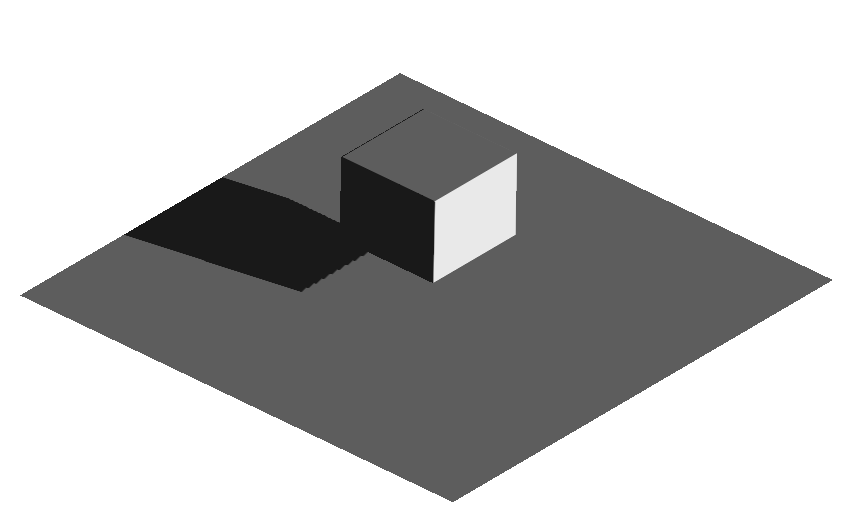
\includegraphics[width=12cm, height=10cm, keepaspectratio=true]{Osencen_model.png}
\end{center}
\caption{Primer osenčenega modela. Luč je na desni strani pred modelom.}
\label{osencenmodel}
\end{figure}

\subsection*{Izris objekta s projicirano sliko}
Za izris s projekcijo moramo, če je delec viden, izračunati kje v sliki se ta delec nahaja, nato pa namesto bele svetlobe vzeti barvo svetlobe, ki je na tem mestu v sliki. Slika \ref{teksturaprojecirananamodel} je primer izrisa s projecirano sliko, kjer je projecirana slika vijolično-siva šahovnica.

\begin{figure}[h]
\begin{center}
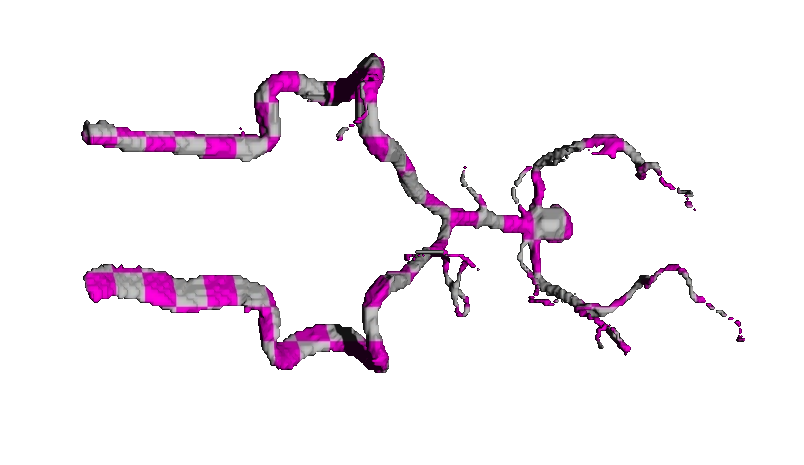
\includegraphics[width=12cm, height=10cm, keepaspectratio=true]{Tekstura_projecirana_na_model.png}
\end{center}
\caption{Primer projekcije teksture na model.}
\label{teksturaprojecirananamodel}
\end{figure}

\section{Nabor podatkov}
3D posnetki so volumetrični posnetki ožilja možganov, narejeni z magnetno resonanco, ki so nato s pomočjo funkcionalnosti že obstoječe aplikacije pretvorjeni v mrežni model, 2D posnetki pa so rentgenski posnetki ožilja shranjeni kot slikovna datoteka tipa jpeg\cite{jpeg}. Volumetrični podatki so shranjeni v datotekah tipa Mhd\cite{mhd}.

\chapter{Implementacija}
\section{Programska ovojnica za LWJGL}

Za lažje delo z OpenGL sem napisal programsko ovojnico, ki temelji na knjižnici LWJGL. OpenGL zahteva veliko vodenja podatkov o stanju, saj je potrebno vsa sredstva, kot so medpomnilniki, senčilniki, teksture in več, ročno uničiti, da se pomnilnik na grafični enoti ne zasiči. Ovojnica to poenostavi tako, da OpenGL sredstva zavije v smiselno poimenovane razrede. Ovojnica nudi tudi transformacije med kvaternioni in evklidskimi koti in razrede za transformacije in kamere.

\begin{figure}[h!]
\begin{center}
\includegraphics[width=16cm, height=20cm, keepaspectratio=true]{class_diagram.png}
\end{center}
\caption{Diagram dedovanja razredov v programski ovojnici.}
\label{classdiagram}
\end{figure}


\subsection*{Medpomnilniki}

Prenašanje podatkov na grafično enoto in z nje v OpenGL poteka prek medpomnilnikov. 

Uporabil sem naslednje OpenGL medpomnilnike:
\begin{description}

\item [Medpomnilnik za sezname] hrani podatke potrebne za izris kot so položaji oglišč, pravokotnice v ogliščih, teksturne koordinate in tudi poljubne podatke, ki jih definira uporabnik.

\item [Medpomnilnik za seznam elementov] grafični enoti pove kako se sestavljajo osnovni liki.

\item [Medpomnilnik za okvirje] je drugačen tip medpomnilnika, saj sam po sebi ne hrani podatkov, vendar določa kam se bodo zapisali podatki iz cevovoda za izris.

\end{description}
Podprti pa so še naslednji tipi medpomnilnikov, ki pa so zunaj obsega predstavljenega dela: za kopiranje, za pakiranje pikslov, za poizvedbe, za teksture, za povratno informacijo o transformacijah, za enotne spremenljivke, za posreden izris, za atomarne števce, za posredno odpremo ukazov in za hranjenje senčilnikov.


Ovojnica podpira medpomnilnike za sezname, ki se uporabljajo za prenašanje podatkov kot so položaji oglišč, normale v ogliščih in teksturne koordinate, medpomnilnike za elemente, ki grafični enoti povedo iz katerih oglišč so sestavljene ploskve, ter medpomnilnike za okvirje (angl. frame), ki hranijo slike za izris.

\subsection*{Senčilniki}

Senčilniki so podprogrami za izris, ki jih mora napisati uporabnik. V starejših različicah se je uporabljal fiksni cevovod za izris, v novejših verzijah pa so nekateri deli programabilni. OpenGL cevovod je sestavljen iz nasledjih faz, prikazanih v sliki \ref{filerenderingpipeline}:

\begin{figure}[h]
\begin{center}
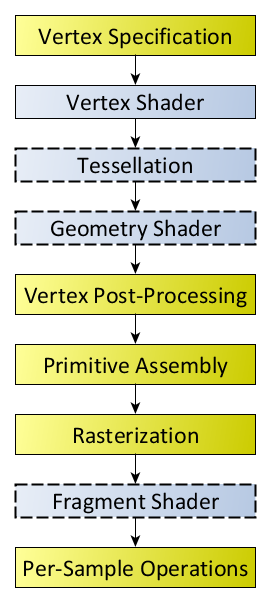
\includegraphics[width=12cm, height=10cm, keepaspectratio=true]{File_RenderingPipeline.png}
\end{center}
\protect\cite{renderingpipelineoverview}
\caption{Skica cevovoda za izris. Rumeni pravokotniki so fiksni deli, modri pa so v novejših različicah programabilni.}
\label{filerenderingpipeline}
\end{figure}


\begin{description}
\item [Specifikacija oglišč] je faza cevovoda, v kateri uporabnik poda seznam oglišč in kako se združujejo v osnovne like kot so točke, črte, trikotniki in seznami trikotnikov.
\item [Senčilnik za oglišča] so uporabniški podprogrami, ki izvajajo poljubne operacije nad posameznimi oglišči. Uporabnik lahko določa izhodne spremenljivke, vendar pa mora med njimi nujno biti položaj. Ta faza cevovoda je obvezna.
\item [Senčilnik za deljenje ploskev] je neobvezen del cevovoda. Uporabnik definira dva senčilnika, senčilnik za nadzor deljenja in senčilnik za izračun deljenja. Prvi lahko deluje samostojno, drugi pa nujno potrebuje še prvega. V senčilniku za nadzor se izračuna kako podrobno se bodo liki delili, v senčilniku za izračun pa se izračunajo novi liki.

\item [Senčilnik za geometrijo] so prav tako neobvezni, definira pa jih uporabnik. Kot vhodne podatke dobijo osnovne like, ki pa jih lahko zavržejo, spremenijo in delijo.

\item [Naknadna obdelava oglišč] je faza, v kateri se liki iz prejšnjih faz zavržejo, če ne spadajo v pogled kamere, oziramo razrežejo, če so delno v pogledu kamere. Po želji se lahko podatki tu shranijo v medpomnilnik, da jih ni potrebno ponovno računati, če se ne bodo spreminjali.
\item [Sestavljanje osnovnih likov] je faza, v kateri se podatki iz prejšnjih faz pretvorijo v osnovne like, ki smo jih hoteli izrisati. Naprimer, če so vhodni podatki trikotniki, želimo pa le izris črt, se bo tu vsak trikotnik razdelil v tri črte. Tu se lahko cevovod konča, če želimo le izračunati podatke za pozneje, ne pa jih tudi izrisati. 
\item [Rasterizacija] je faza, kjer se osnovni liki razdelijo v diskretne delce, ki služijo izračunu končne barve piksla.
\item [Senčilnik za drobce]izračuna barvo piksla in njegovo globina. Ta del cevovoda je neobvezen, vendar se, če ga ni, izračuna le globina delca.
\item [Procesiranje drobcev] je faza kjer se, če uporabnik tako nastavi, določi kateri delci, izmed tistih na istem položaju, se bodo obdržali glede na globino, šablono in druge lastnosti. Na koncu se barve prosojnih delcev zmešajo, nato pa se rezultat zapiše na zaslon ali v medpomnilnik za okvirje.
\end{description}

Poleg teh senčilnikov OpenGL podpira še senčilnike za izračun, ki pa se ne izvajajo v cevovodu in so namenjeni izračunu poljubnih podatkov.

Ovojnica podpira pet vrst senčilnikov, in sicer senčilnike za oglišča (angl. vertex shader), za geometrijo (angl. geometry), za drobce (angl. fragment) in za deljenje (angl. tesselation), obstaja pa še senčilnik za izračunavanje (angl. compute shader), ki pa ni podprt. Senčilniki se združujejo v programe, ki tvorijo programabilen del cevovoda za izris.

\subsection*{GLSL}

OpenGL senčilniki se pišejo v jeziku GLSL\cite{GLSL} (angl. OpenGL Shading Language). GLSL je osnovan na jeziku C in omogoča prenosljivost med operacijskimi sistemi in različnimi proizvajalci strojne opreme.

\subsection*{Teksture}

Teksture v OpenGL so objekti, ki vsebujejo eno ali več slik, ter so uporabni kot vir slikovnih podatkov v senčilnikih ali kot tarča za izris v medpomnilnikih za okvirje. Ker je inicializacija teksture v OpenGL precej kompleksna, ovojnica poskrbi za inicializacijo osnovnih parametrov.

OpenGL podpira naslednje tipe tekstur:

\begin{description}
\item [1D, 2D in 3D teksture]so teksture, kjer so slike shranjene v 1, 2 ali 3 dimenzionalnih poljih.
\item [Pravokotna teksture]so teksture, ki so nujno dvodimenzionalne in imajo drugačne metode za dostop do podatkov.
\item [\textcolor{red}{Kockaste teksture}]so teksture, sestavljene iz šestih enako velikih kvadratnih tekstur.
\item [Večvzorčne teksture]so teksture, ki za izračun vsakega piksla izračunajo več vzorcev, kar omogoča lepši izris.
\item [Seznami tekstur]so teksture, ki vsebujejo sezname slik. Podprte so 1D, 2D, kockaste in večvzorčne teksture.
\end{description}

Ovojnica podpira le 2D teksture, ostale pa v aplikaciji niso uporabljene.

\subsection*{Točkovni nizi}

Točkovni nizi (angl. vertex array object) so OpenGL objekti, ki hranijo stanje potrebno za izris objektov. Hranijo le stanje, ne pa tudi samih podatkov, to je reference na medpomnilnike in obliko podatkov v teh medpomnilnikih, ne pa tudi samih podatkov iz medpomnilnikov. Prednost se kaže v hitrosti in velikosti kode, saj je potrebno veliko manj sprememb stanja.

\subsection*{Transformacija}

Transformacija (angl. transform) je razred, ki je namenjen hranjenju transformacije objekta, to je rotacija, položaj in velikost. Položaj in velikost sta predstavljena kot vektorja dolžine 3, rotacija pa kot kvaternion. Podprte so rotacije in premiki v lokalnem ter globalnem koordinatnem sistemu, ter rotacije v poljubnem sistemu. Razred vsebuje tudi funkcije za pretvorbo iz kvaternionov v eulerjeve kote, za izračun transformacijske matrike iz stanja transformacije, ter za izračun kvaterniona iz rotacijske matrike.

(Formule za pretvorbe?)

Kot posebna transformacija se obravnava tudi kamera, le da so pri kameri premiki ravno obrnjeni, ima pa še dodatne parametre za pogled kamere. Podprti sta dve vrsti kamere: perspektivna in vzporedna.
\subsection*{Izjeme}
Ovojnica podpira več vrst izjem. OpenGL sam ne ustavi izvajanja programa ob napaki, vendar pa je izris nepravilen, zato ob nekaterih operacijah ovojnica preverja, če je na grafični enoti vse v redu. Izjeme se lahko prožijo, ko se senčilnik ne prevede pravilno, ko se program ne poveže pravilno ali ko se medpomnilnik za okvirje ne inicializira pravilno.

\subsection*{Ostalo}

Poleg že naštetega ovojnica vsebuje še funkcijo za razhroščevanje, ki napake, ki jih vrača OpenGL, pretvori v berljive nize ter izpiše vrstico v kateri je bila funkcija klicana, kar močno olajša iskanje napak.

\section{Samostojna aplikacija}

Funkcionalnost orodja sem najprej implementiral kot samostojno aplikacijo, saj je tako lažje preveriti pravilnost delovanja. Aplikacija nima uporabniškega vmesnika, implementiran pa je le osnovni uporabniški nadzor, saj služi le kot primer delovanja, ne pa tudi dejanski uporabi. Sestavljena je iz testnega razreda, razreda ki implementira dejansko funkcionalnost in razredov za branje Obj datotek, ki pa niso uporabljeni v končni aplikaciji, saj ima ta svoj bralnik. Posnetki se v samostojni aplikaciji ob zagonu naložijo avtomatsko iz testnih datotek.

\begin{figure}[h]
\begin{center}
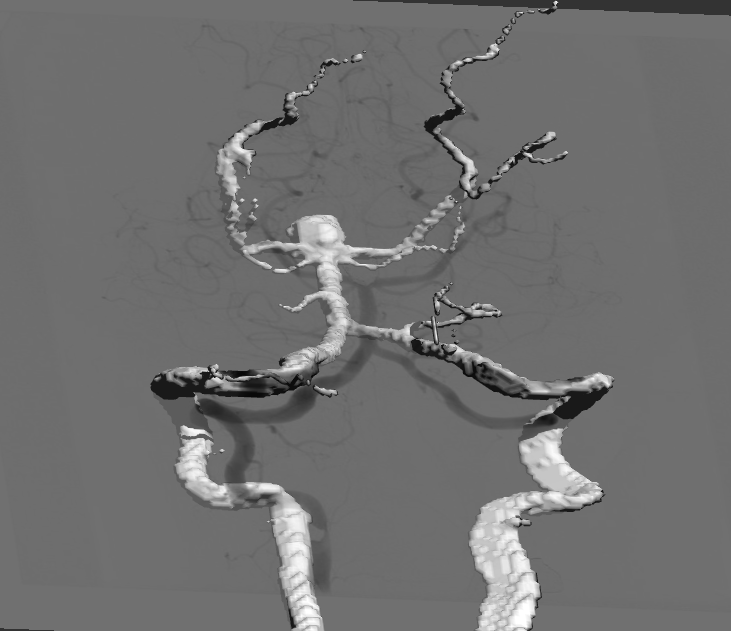
\includegraphics[width=12cm, height=10cm, keepaspectratio=true]{Samostojna_aplikacija.png}
\end{center}
\caption{Pogled samostojne aplikacije.}
\label{samostojnaaplikacija}
\end{figure}

\subsection*{Premikanje pogleda}

Aplikacija podpira dva pogleda, pogled iz kamere ter pogled iz projektorja. Pogled iz kamere je glavni pogled, v katerem naj bi si uporabnik ogledoval model, na katerega je projicirana tekstura. V tem pogledu je mogoče s kamero poljubno premikati in krožiti okrog modela in projektorja, medtem ko sta ta pri miru. Pogled iz projektorja je namenjen poravnavi projicirane teksture z modelom. V tem pogledu se prizorišče izrisuje iz iste smeri kot sveti projektor, s premikanjem le-tega pa uporabnik poravnava 2D in 3D posnetka.

\subsection*{2D posnetek}

Dvo dimenzionalni posnetek je rentgenska slika ožilja. Slika se projecira na pravokotnik, ki je prilagojen velikosti slike. Sliko se da v prostoru rotirati neodvisno od modela, kar služi poravnavi, ko pa sta model in slika poravnana, se lahko rotira skupaj z modelom.

\subsection*{3D posnetek}

Tri dimenzionalni posnetek je mrežni model ožilja, naložen iz Obj datoteke. 3D posnetek se sam po sebi ne premika, premika se le kamera, kar pa da uporabniku podoben vtis.

\section{Integracija v aplikacijo za vizualizacijo}

Za konec sem funkcionalnost integriral še v aplikacijo za vizualizacijo. Poleg funkcionalnosti samostojne aplikacije je bilo potrebno zagotoviti, da se modul obnaša čim bolj podobno že obstoječi aplikaciji, kar pa ni bilo čisto mogoče, saj modul uporablja drugačno vrsto kamere kot preostala aplikacija. 

\subsection*{Premikanje pogleda}

Model žil se premika enako kot v že obstoječi aplikaciji, s smernimi tipkami za premik levo, desno, naprej in nazaj ter s tipkama 'r' in 'f' za gor in dol. Obrača se s tipkami 'w', 'a', 's', 'd', 'q' in 'e' ter z miško, tako da se lev miškin gumb drži nad objektom in miško premika. Premikanje z miško je, podobno kot v že obstoječi aplikaciji, narejeno s projekcijo kazalca na navidezno kroglo okoli modela, vendar pa je zaradi drugačne vrste kamere izračun preseka drugačen. (*matematika za izračunom*) 


\subsection*{Nalaganje datotek}
Funkcionalnost za nalaganje datotek je obstajala že v osnovni aplikaciji. Uporabnik s pritiskom na gumb \emph{'odpri'} dobi pojavno okno, v katerem izbira datoteke. Podprti formati so bili mhd za volumetrične datoteke, ter Obj za mrežne modele. Moral sem dodati še možnost za nalaganje slikovnih datotek v standardnih formatih jpeg in png \cite{png}. Java podpira ta dva formata v svoji standardni knjižnici, tako da je bila implementacija preprosta.

\chapter{Zaključek}
\textcolor{red}{V diplomskem delu sem implementiral projekcijo 2D rentgenske slike na 3D mrežni model. Vhodni podatki so mrežni modeli v datotekah tipa Obj in rentgenske slike tipa obj. Mrežni modeli so bili pretvorjeni iz MHD datotek v mrežne modele v okviru že obstoječe aplikacije Neck veins.
}

\textcolor{red}{Implementacija je bila napisana v programskem jeziku Java, kar je omogočilo brezhibno integracijo v že obstoječo aplikacijo. Za lažji in hitrejši razvoj sem razvil še programsko ovojnico za LWJGL, ki hrani stanje OpenGL objektov in ima bolj berljivo poimenovane funkcije.}

\textcolor{red}{V okviru nadaljnjega dela bi lahko implementiral algoritem za avtomatsko poravnavo 2D in 3D posnetkov\cite{6507588}, razvit na FRIju.}

\bibliographystyle{plain}
\bibliography{literature}
\end{document}